\chapter{Literatuurstudie}
\section{Inleiding}
%%% Leuke insmijter waarbij vertelt wordt dat software deployment oud is
In dit hoofdstuk, wordt een bespreking gegeven over alle mogelijke technieken, technologieën, architecturen, \ldots die een oplossing kunnen bieden voor het probleem dat in het vorige hoofdstuk besproken werd.
Eerst wordt het deploymentproces besproken en wordt nagegaan welke problemen hiermee geassocieerd worden.
Vervolgens worden enkele case studies besproken om een beeld te krijgen van alle verschillende tools die aanwezig zijn en die gebruikt kunnen worden om het probleem omtrent het verspreiden van de software van de producent naar de gebruiker op te lossen.
Na de cases studies worden ook enkele architecturen besproken die gebruikt kunnen worden om een applicatie te ontwerpen die om kan gaan met een groeiend aantal gebruikers.
Hierna wordt nagegaan op welke manier een ``rampenplan'' geïmplementeerd kan worden zodat de problemen die ontstaan tijdens het deploymentproces opgelost kunnen worden.
Uit de probleembespreking is ook gebleken dat er nood is aan een applicatie die overweg kan met verschillende programma's die Televic gemaakt heeft of nog zal maken.
Om te achterhalen wat mogelijk is om dit te realiseren, worden verscheidene technologieën besproken die hiervoor een oplossing kunnen bieden.

\section{Software deployment}\label{sec:softwareLevenscyclus}
De levenscyclus van software deployment kan volgens \citet{softwareDeployment,hall1999cooperative} beschreven worden in verschillend stappen, namelijk:
\begin{itemize}
\item \emph{Release}: de software is volledig samengesteld uit pakketten die voldoende metadata bevatten om de verschillende bronnen te beschrijven waarvan het pakket afhangt.
\item \emph{Installatie}: de software moet overgebracht worden naar de gebruiker en geconfigureerd worden in voorbereiding op de activatie.
\item \emph{Activeren}: tijdens de activatie wordt de software-uitvoering opgestart of worden de nodige triggers geplaatst om de executie op het gepaste tijdstip op te starten.
\item \emph{Deactiveren}: dit is het tegengestelde van activeren. Deze stap is nodig zodat een aanpassing of herconfiguratie uitgevoerd kan worden.
\item \emph{Updaten}: dit is het proces waarin de software wordt aangepast. Deze stap wordt vaak geactiveerd door het uitbrengen van een nieuwe versie van de software.
\item \emph{Deïnstallatie}: tijdens deze stap zal de geïnstalleerd software van het gebruikerssysteem gehaald worden.
\end{itemize}
De enige fase van de levenscyclus die zich uitsluitend op de server afspeelt is de release fase.
De rest van de fases spelen zich af op de verschillende gebruikerssystemen.

\begin{figure}[!ht]
\centering
\makebox[0pt]{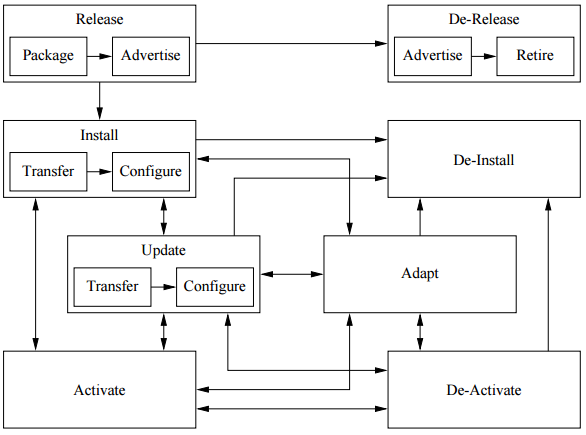
\includegraphics[scale=0.7]{afbeelding/softwareLevenscyclus.png}}
\caption{De levenscyclus van software \citep{carzaniga1998characterization}}
\label{fig:softwareLevenscyclus}
\end{figure}

In theorie zou het deployen van software een eenvoudige klus moeten zijn.
Aangezien software bestaat uit een set van bestanden, zou het deployen van software naar een doelcomputer slechts bestaan uit het kopiëren van de nodige bestanden.
Maar dit is vaak niet het geval.
Volgens \citet{dolstra2006purely} zijn er in de praktijk verschillende oorzaken die aan de basis liggen van een ingewikkeld deploymentproces.
Deze oorzaken kunnen in twee grote categorieën ingedeeld worden, namelijk de omgevings- en de onderhoudsproblemen.

\paragraph{Omgevingsproblemen}
In de eerste categorie ligt de nadruk vooral op correctheid.
Voordat de software geïnstalleerd wordt op een doelsysteem, wordt de doelomgeving ondervraagd naar alle eigenschappen: zijn de nodige programma's aanwezig, bestaan alle configuratiebestanden, \ldots .
Als deze eisen niet voldaan zijn, dan zal de software niet correct werken.
\citet{dolstra2006purely} haalt enkele concrete voorbeelden aan van omgevingsproblemen:
\begin{itemize}
\item De deployment van software kan een gedistribueerd probleem opleveren.
Software kan afhankelijk zijn van componenten draaiende op externe systemen of van andere processen draaiende op het doelsysteem.  
\item Software is vaak afhankelijk van verschillende andere softwarecomponenten. 
Deze afhankelijkheden (dependencies) moeten voor de deployment bepaald worden.
Dit proces is moeilijk en een fout kan pas laat ontdekt worden.
\item De afhankelijkheden moeten compatibel zijn met wat de software verwacht.
Bepaalde versies van een afhankelijkheid zijn compatibel met de software terwijl andere versies dit niet zijn.
Dit komt doordat sommige depencies build-time variaties vertonen.
At build-time worden bepaalde eigenschappen geselecteerd met als gevolg dat de dependency meer of minder functionaliteiten bevat ten opzichte van een vorige build.
\item Sommige softwarecomponenten zijn afhankelijk van specifieke hardware.
Dit kan enkel verholpen worden door op voorhand te controleren welke hardware aanwezig is.
\end{itemize}

Uit deze concrete voorbeelden wordt al snel duidelijk dat er twee problemen zijn: de verschillende eisen van de software moeten geïdentificeerd worden en vervolgens moet aan deze eisen voldaan worden in het doelsysteem.

\paragraph{Onderhoudsproblemen}
Naast de verschillende omgevingsproblemen, beschrijft \citet{dolstra2006purely} ook enkele onderhoudsproblemen.
Deze hebben te maken met het feit dat software moet kunnen ``evolueren''.
Om dit te ondersteunen, moeten allerlei actie zoals upgraden en updaten uitgevoerd worden.
Enkele voorbeelden van zulke acties zijn:
\begin{itemize}
\item Tijdens het verwijderen van software moeten alle componenten verwijderd worden.
Er mogen echter geen componenten verwijderd worden die nog in gebruik zijn door andere software.
\item Ook tijdens het updaten van software moet rekening gehouden worden met andere software.
Het updaten van een component kan voor problemen en failure zorgen in een andere component.
Een DLL-hell wordt best vermeden.
\item Na het upgraden/updaten van een component, is het soms aangewezen om een rollback uit te voeren.
Zo'n actie kan overwogen worden als na de upgrade belangrijke functionaliteiten van de software niet meer functioneren.
\end{itemize}

\section{Case studies}\label{sec:caseStudies}
Uit de vorige sectie blijkt dat het software-deploymentproces een uitgebreid en ingewikkeld proces is.
Er moet rekening gehouden worden met verscheidene stappen die elk een eigen doel en functie hebben, maar ook met verschillende problemen die kunnen optreden voor, tijdens en na deze stappen.
Door de jaren heen zijn er verschillende technologieën ontwikkeld die het probleem van software deployment aanpakken.
In wat volgt, worden enkele van deze technologieën besproken en wordt nagegaan op welke manier zij software-deployment aanpakken.
Op deze manier wordt een beeld gecreëerd van de mogelijke technologieën die gebruikt kunnen worden om de software van Televic van de producenten naar de gebruikers te krijgen.

%\subsection{Java Beans}
%Enterprise JavaBeans (EJB) zijn een standaard voor het bouwen van server-side componenten.
%De EJB's zijn speciaal ontworpen voor het vereenvoudigen van de deployment.
%\citet{softwareDeployment} beschrijft JavaBeans als eenheden van business logic in een component die uitgevoerd wordt in een container.
%De verschillende containers zorgen voor een abstractie van de hosting omgeving en bieden verscheidene services aan.
%Een JavaBean moet ingepakt worden volgens de specificaties die Sun Microsystems oplegt.
%Met deze standaard is het mogelijk om verschillende management en deployment tools te schrijven die de EJB's kunnen beïnvloeden.
%Enterprise JavaBeans worden ingepakt in de standaard Java JAR file, samen met een XML deployement descriptor.
%De descriptor beschrijft de verschillende eigenschappen van de bijhorende EJB.
%
%De Enterprise JavaBeans zijn volgens \citet{softwareDeployment} fijnkorrelige en taalafhankelijke oplossing voor het deployment probleem.
%Door het isoleren van de Beans door middel van een gestandaardiseerde container interface zullen Enterprise JavaBeans zo een oplossing vinden voor het deployment probleem.
%Hierdoor moeten de EJB's zodanig ontworpen worden dat ze voldoen aan de eisen van de interface.
%Enterprise JavaBeans hebben geen idee van het op afstand installeren van componenten.
%Een groot probleem bij EJB's is dat referenties naar afhankelijke beans gebeurd via niet unieke namen.
%Twee verschillende beans met eenzelfde naam moeten hierdoor manueel herladen worden zodanig dat de bindings up-to-date zijn \citep{rutherford2002reconfiguration}.
\subsection{Electric cloud}
%%% TODO
%http://electric-cloud.com/wp-content/uploads/Ovum-Decision-Matrix-Selecting-DevOps-Release-Management-Solution-2016-2017-print.pdf
%https://www.gartner.com/doc/reprints?id=1-3DSWYP2&ct=160801&st=sb
Electric cloud is een bedrijf opgericht in 2002 met een focus op application release automation (ARA).
Hun product, ElectricFlow, is ontworpen om het beschikbaar stellen, het bouwen en het verspreiden van mutlitiered applicaties te vereenvoudigen.
Dit gebeurt aan de hand van de model-driven architectuur \citep{gartner}.
\citet{electricflow} beschrijft ElectricFlow als een enterprise-grade DevOps Release Automation platform.
Met behulp van de model-driven aanpak is het mogelijk voor gebruikers om meerde pipelines en releases over verschillende infrastructuren te coördineren op een eenvoudige manier.

De kern van ElectricFlow bestaat uit een web-based systeem dat gebruikt wordt voor het automatiseren en het onderhouden van het bouw-, test-, deployment en releaseproces.
Het automatiseringsplatform bestaat uit een drie-lagen architectuur, een web interface en mogelijkheden om build en release analyses uit te voeren.
De drie-lagen architectuur van ElectricFlow bestaat uit:
\begin{itemize}
\item \textbf{ElectricFlow Server}: een server die instaat voor het managen van resources, commando's en het generen van rapporten.
\item \textbf{Databank}: een databank die instaat voor het opslaan van commando's, meta-data en logfiles.
\item \textbf{Agents}: verschillende agenten die instaan voor het uitvoeren van commando's, het monitoren van statussen en het verzamelen van resultaten.
\end{itemize}
Figuur~\vref{fig:electricflowArchitecture} geeft de architectuur weer van ElectricFlow.
In de figuur zijn de verschillende lagen zichtbaar samen met de verschillende andere tools die vervat zitten in het automatiseringsplatform \citep{electricflow}.

\begin{figure}[!ht]
\centering
\makebox[0pt]{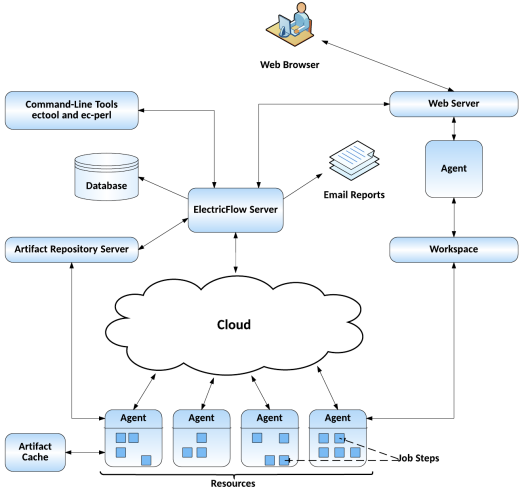
\includegraphics[scale=0.9]{afbeelding/electricflowArchitecture.png}}
\caption{ElectricFlow Architectuur \citep{electricflow}}
\label{fig:electricflowArchitecture}
\end{figure}

Om ElectricFlow te gebruiken voor bouw en test automatie, is het nodig om de volgende objecten te creëren, te configureren en bij te houden.
\begin{itemize}
\item \textbf{Project}: een project in ElectricFlow dient als container waarin procedures, stappen, workflows, \ldots zitten.
Op deze manier is het mogelijk om een scheiding te creëren tussen projecten die bijvoorbeeld een ander doel hebben.
\item \textbf{Resource}: een resource wordt gedefinieerd als een agent machine waar stappen in uitgevoerd kunnen worden.
\item \textbf{Procedures}: procedure en stappen worden gebruikt om taken in ElectricFlow te definiëren.
Een procedure bestaat uit één of meerdere stappen waarbij in ieder stap een commando of script wordt uitgevoerd.
\item \textbf{Workflow}: een workflow stelt de gebruiker in staat om build-test-deploy levenscycli te definiëren.
Zo wordt het managen van verschillende procedures en stappen in een project eenvoudiger.
\end{itemize}

Met ElectricFlow is het mogelijk om verscheiden applicaties op een autonome wijze te verschepen naar de gebruikers.
Hierbij kan door middel van een procedure een gepersonaliseerde afhandeling plaatsvinden.
Door gebruik te maken van de verscheidene projecten is het mogelijk om de release van verschillende applicaties op een geordende manier aan te pakken. 
Verder wordt niks vermeld over hoe omgegaan wordt met installaties en updates die slecht zijn afgelopen.

\subsection{Redhat package manager}
In Linux wordt de Redhat package manager (RPM) het vaakst gebruikt voor de deployment van software.
Met hulp van RPM is het mogelijk om enkele operaties uit te voeren zoals onder andere installatie, updaten, \ldots .
De operaties worden ondersteund door een databank die alle informatie en details van de geïnstalleerde pakketten bevat.
Een RPM pakket bestaat uit executables gecombineerd met configuratiebestanden en documentatie.
Doordat een pakket executables bevat, zal een pakket gekoppeld zijn aan het besturingssysteem van de host \citep{bailey1997maximum}.
Naast de RPM files bevat een pakket verschillende scripts geschreven in de standaard Unix scripting taal.
De verscheidene scripts zijn ingedeeld in sets horende bij een specifieke taak.
Bij een error moet een roll back uitgevoerd worden.
Dit is de taak van de script schrijver \citep{softwareDeployment}.

De Redhat Package Manager is een grofkorrelige, taal onafhankelijke maar besturingssysteem afhankelijke oplossing.
Het grootste probleem van RPM schuilt in de afhankelijkheden tussen de pakketten.
Niet alle afhankelijkheden zijn expliciet gemodelleerd en de afhankelijkheden die wel gemodelleerd zijn, zijn gevormd met de nadruk op de inhoud en niet op de pakketten zelf \citep{softwareDeployment}.  

\subsection{ATLAS}\label{sec:ATLAS}
ATLAS is één van de vier grote experimenten bij de Large Hadron Collider (LHC) in CERN (de Europese organisatie voor nucleair onderzoek).
%Het is een algemeen deeltjesfysica experiment onderhouden door een internationale samenwerking met als doel het exploiteren van de mogelijkheden van de Large Hadron Collider.
%Fysici testen de voorspellingen van het Standaard Model \cite{standardModel} wat kan leiden tot grote ontdekkingen zoals het Higgs  boson \cite{atlas}.

Om in de ATLAS-samenwerking (specifiek voor het LCG/EGEE project, LHC Computing Grid/Enabling Grids for E-sciencE \citep{bird2005lhc}) om te gaan met de grote hoeveelheid bronnen, is er een volledig automatisch installatiesysteem ontworpen. 
\citet{salvo2008atlas} beschrijft de architectuur van het ontworpen systeem.
Het ontwerp van het installatiesysteem werd gebaseerd op het Light Job Submission Framework for installation, ook wel LJSFi.

\begin{figure}[!ht]
\centering
\makebox[0pt]{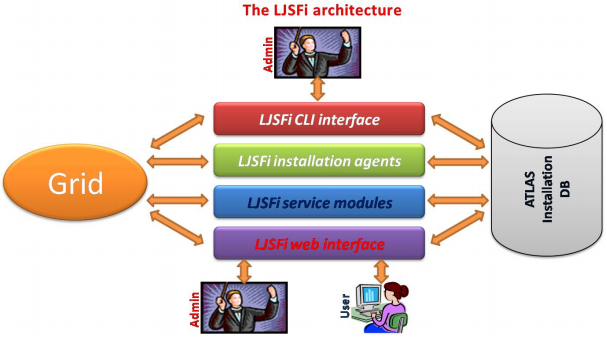
\includegraphics[scale=0.7]{afbeelding/ljsfiArchitectuur.png}}
\caption{LJSFi Architectuur \citep{salvo2008atlas}}
\label{fig:ljsfiArchi}
\end{figure}

De architectuur van het framework is zichtbaar in Figuur~\ref{fig:ljsfiArchi}.
Het framework vormt een dunne laag over de middleware van Grid (Grid is een gedistribueerde computerinfrastructuur voor geavanceerde wetenschappen. De focus ligt bij het delen van resources en innovatieve applicaties.\citep{foster2001anatomy}).
De kern van het systeem bestaat uit de installatiedatabase en de command line interface (CLI).
De laatste zorgt voor de interacties met de Grid middleware.
Met hulp van de installatiedatabase kan de CLI de verschillende taken en de job informatie opslaan.
Aan de hand van deze informatie kunnen installaties uitgevoerd worden.
De installatiedatabank staat in contact met alle componenten van het framework.
Zo kan de status van verscheidene acties en configuraties van verschillende taken opgeslagen worden.

Naast deze twee grote componenten bevat LJSFi servicemodules en extensies waarmee installatie aanvragen afgehandeld worden.
Het systeem bevat drie verschillende componenten die horen bij de LJSFi service modules:
\begin{itemize}
\item \textbf{RAI module} De Request An Installation module dient als web interface voor het ontvangen van user-driven installatie-aanvragen.
\item \textbf{AIR module} De Automatic Installation Requester schiet in actie als de software release aangeduid staat als productie of veroudert en als de release aangeduid staat met de parameter auto-installatie.
De module zal respectievelijk de software installeren of verwijderen op alle sites waar de software tag nog niet aanwezig is.
Door de AIR module periodiek te gebruiken, zullen de nodige aanvragen snel afgehandeld worden.
\item \textbf{InAgent module} Met de InAgent module wordt het mogelijk om volledig geautomatiseerde installatieprocessen te voorzien.
Iedere 10 minuten wordt de installatiedatabase gelezen en via de CLI interface worden de nodige installatieprocessen opgestart.
Elk installatieproces wordt bijgestaan door een installatie agent.
De agent zal instaan voor het updaten van de installatiedatabase met real-time informatie die online zichtbaar is.
\end{itemize}

Naast de verscheidene automatische services biedt LJSFi enkele gebruikerservices aan.
Een gebruiker kan zich inschrijven voor bepaalde acties op een doelsysteem.
Als deze actie wordt uitgevoerd dan krijgt de gebruiker een mail.
Hiernaast kan een gebruiker een software release vastpinnen zodat deze niet verwijderd kan worden door het systeem.

Het installatieproces wordt uitgevoerd in drie verschillende stappen.
In een eerste stap wordt een sitecontrole uitgevoerd door een piloot taak naar de site te sturen.
Als de check succesvol uitgevoerd wordt, kan het installatieproces beginnen.
De acties tijdens het installatieproces worden uitgevoerd door softwaremanagementscripts.
Op het einde van het proces, haalt het systeem de joboutput en exit-code op.
De laatste wordt opgeslagen in de installatiedatabase.

\citet{Obreshkov2008244} bespreken hoe het ATLAS project te werk gaat bij het inpakken van alle nodige software.
Het ATLAS project gebruikt CMT \citep{cmt} als configuratie manager.
Met behulp van een configuratie bestand weten verscheidene tools hoe ze een pakket moeten afhandelen.
\citet{packAtlas} spreekt ook over CMT als informatiebron voor het ophalen van meta-data.
Aan de hand van deze data kan een Pacman pakket geproduceerd worden.
Met behulp van een ``Pacman file'' is geweten hoe de ingepakte software behandeld moet worden.

De LJSFi architectuur is een architectuur die om kan gaan met een grote hoeveelheid pakketten.
Door gebruik te maken van de modules is het mogelijk om de verschillende pakketten te installeren en te verwijderen op een grote schaal zonder dat menselijke interactie nodig is.
Hierbij zorgt CMT voor de nodige meta-data waardoor installatietools niet afhankelijk zijn van de mens.
Een nadeel aan deze architectuur is dat het gebruik van Grid nodig is om de LJSFi architectuur in te bouwen.
Verder wordt in de lectuur niet ingegaan op welke wijze er wordt omgegaan met een fout tijdens het installatieproces of het verwijderproces.
Het enige dat hierover vermeld wordt is dat de exit-code van de job niet rechtstreeks gebruikt worden.

\subsection{ORYA}\label{sec:ORYA}
\citet{lestideau2003providing} leggen uit hoe ORYA (Open enviRonment to deploY Applications) verschillende deployment functionaliteiten aanbiedt aan gedistribueerde, autonome entiteiten zoals workstations en servers.
Aan de hand van een deployment PSEE \citep{belkhatir2007adele} wordt het mogelijk om het installatieproces te automatiseren.

In het ontwerp van ORYA worden er drie verschillende entiteiten besproken die nodig zijn om het automatische installatieproces mogelijk te maken.
\begin{itemize}
\item \textbf{Applicatie Server} De applicatie server bevat de informatie nodig voor de installatie.
Hieronder bevindt zich onder andere een pakket met de nodige resources en een manifest waarin de afhankelijkheden, beperkingen en kenmerken staan.
\item \textbf{Target} De target is het doel waarop de deployment uitgevoerd wordt.
Iedere target wordt beschreven door de verschillende applicaties die al aanwezig zijn en de fysische beschrijving.
\item \textbf{Deployment Server} De deployment server vormt de kern van de deployment omgeving en staat in voor het uitvoeren van de deployments. 
De deployment server zoekt de nodige pakketten, voert een transfer van de pakketten uit en installeert de applicatie.
Op het einde moet de deployment server garanderen dat andere programma's correct blijven functioneren.
\end{itemize}

\citet{lestideau2003providing} beschrijven verder de verschillende modellen die gehanteerd worden om een succesvolle deployment uit te voeren.
In Figuur~\ref{fig:deploymentModel} is het deployment-procesmodel terug te vinden.
Een deploymentproces zal bestaan uit verschillende basisactiviteiten en deploymentprocessen.
Iedere activiteit wordt uitgevoerd door een agent.

\begin{figure}[!ht]
\centering
\makebox[0pt]{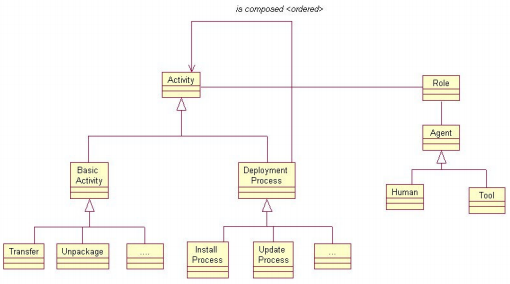
\includegraphics[scale=1]{afbeelding/deploymentModelORYA.png}}
\caption{Deployment-procesmodel \citep{lestideau2003providing}}
\label{fig:deploymentModel}
\end{figure}

Een toegepast voorbeeld van een deployment aan de hand van dit model is terug te vinden in Figuur~\ref{fig:deploymentVoorbeeld}.
Een basisactiviteit wordt voorgesteld aan de hand van een grijze rechthoek en een deploymentproces aan de hand van een witte rechthoek.
In het voorbeeld zijn dus vier deploymentprocessen aanwezig en 3 basisactiviteiten.

\begin{figure}[!ht]
\centering
\makebox[0pt]{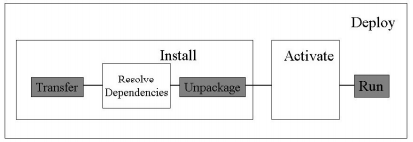
\includegraphics[scale=0.7]{afbeelding/deploymentVoorbeeld.png}}
\caption{Voorbeeld van een deployment \citep{lestideau2003providing}}
\label{fig:deploymentVoorbeeld}
\end{figure}

Aan de hand van deze structuur wordt het mogelijk om het volledige deploymentproces voor te stellen.

%\subsection{Unix}
%\citet{dolstra2006purely} bespreekt Nix deployment systeem omgaan met het deployment probleem.
%Nix houdt verschillende componenten bij in de component store waarbij iedere component een set van bestanden is.
%De componenten worden van elkaar gescheiden door een unieke naam.
%Dit wordt bekomen door een cryptografische hash op te nemen in de naam.
%Unix biedt geen software deployment aan.
%Het biedt verscheidene mechanismen aan waarmee verschillende deployment beleid beschikbaar worden.
%Met de volgende deployment models is het mogelijk om in Unix de Unix expressies (de bouwstenen van de Unix componenten) te verspreiden:
%\begin{itemize}
%\item \textbf{Handmatige download} Een gebruiker kan zelf pakketten downloaden in de vorm van tar archieven, deze zelf uitpakken en vervolgens installeren.
%Deze strategie is arbeidsintensief en maakt het moeilijk om alles up-to-date te houden. 
%\item \textbf{Updaten aan de hand van een versie management systeem} Een andere strategie is het gebruik van een versie management systeem.
%Hiermee is het up-to-date houden van de pakketten zeer eenvoudig.
%\item \textbf{Kanalen} Een verdere uitbreiding zijn de kanalen.
%Een kanaal is een URL naar een tar archief die de nodige Unix expressies bevat.
%Met deze strategie is het even eenvoudig om pakketten te installeren en up-to-date te houden.
%\item \textbf{One-click installatie} Als er enkel één pakket geïnstalleerd moet worden, dan is de one-click installatie de eenvoudigste optie.
%Via de website van de verdeler kan een link gebruikt worden om het nodige pakket te installeren.
%\end{itemize}

\subsection{Ansible}
Als laatste case studie wordt Ansible besproken.
Ansible is een open source IT configuratiemanagement-, deployment- en organisatietool.
De architectuur van Ansible bestaat uit een agentless push model.
Dit wil zeggen dat er geen additionele software nodig is op de clienttoestellen.
Dit wordt gerealiseerd door gebruik te maken van de remote manegement frameworks aanwezig op de toestellen, SSH voor Linux en Unix en WinRM voor Windows.
Door geen agents te gebruiken, zal Ansible geen resources gebruiken zolang de Ansible het systeem niet aan het gebruiken is \citep{ansible}.

\citep{ansible} beschrijft verder dat Ansible gebruik maakt van \emph{Playbooks} voor de organisatie van de IT omgevingen.
Playbooks zijn YAML\footnote{Een human-readable data serialisatie taal (Een superset van JSON)} definities van taken die beschrijven hoe een taak moet geautomatiseerd worden.
Een Playbook bestaat uit een aantal ``plays'' die uitgevoerd kunnen worden op een set van hosts, ook wel een ``inventory'' genoemd.
Iedere play bestaat uit een set van taken die op een subset van de inventory uitgevoerd kan worden.
Een taak bestaat uit Ansible modules (Een klein stuk code met een specifieke taak).

Hiernaast is het mogelijk om de mogelijkheden van Ansible uit te breiden.
Modules kunnen zelf geschreven worden in eender welke taal met als enige beperking dat een JSON bestand als input en output gebruikt moet worden.
De inventory van een Playbook kan dynamisch ontdekt worden at runtime.
In tegenstelling tot ATLAS en Electric Cloud bevat Ansible geen agenten die gebruikt worden om het deploymentproces in goede banen te leiden.
Wederom is het niet duidelijk wat er gebeurt mochten er fouten optreden tijdens het installatieproces of updateproces.

\section{Recovery na fouten}\label{sec:rollback}
Tijdens de bespreking van het probleem in Sectie~\ref{sec:probleem} werd al aangehaald dat een soort van ``rampenplan'' voorzien moet worden.
Zowel omgevingsproblemen als onderhoudsproblemen (zie Sectie~\ref{sec:softwareLevenscyclus}) kunnen tijdens één van de toestanden in de deployment levenscyclus optreden.
Voor Televic is het niet wenselijk dat een probleem tijdens één van deze toestanden ervoor zorgt dat hun software niet meer correct functioneert aangezien dit kan leiden tot het stilleggen van de productie.
Daarom wordt in de volgende secties verschillende mechanismen besproken waarmee de verscheidene problemen aangepakt kunnen worden.
In wat volgt, wordt vooral rekening gehouden met mechanismen die gebruikt kunnen worden als het probleem zich al voor heeft gedaan.
Deze strategieën zullen typisch proberen terug te keren naar een vorige correct werkende toestand van de software.
De actie waarbij wordt teruggekeerd naar een vorige toestand wordt ook wel rollback genoemd.

\subsection{Rollback strategieën}
\citet{srinivasan2004flashback} spreken over drie manieren waarop rollback strategieën geïmplementeerd worden in hedendaagse systemen.
Checkpointing, main-memory transactions en software rejuvination zijn strategieën die vaak gebruikt worden.

\paragraph{Checkpointing}
Checkpointing is een eenvoudige recovery-strategie.
De toestand van een programma wordt periodiek opgeslagen in een bestand op een extern opslagmedium.
Deze kan, na het falen van het programma, gebruikt worden om te herstellen \citep{plank1994libckpt}.
Bij een checkpointing systeem wordt de volledige toestand van het programma opgeslagen.
Dit zorgt voor een verhoogde overhead waardoor het niet mogelijk is om frequent een checkpoint uit te voeren \citep{srinivasan2004flashback}.

Door gebruik te maken van incrementele checkpoints is het evenwel mogelijk om dit probleem aan te pakken.
Enkel de veranderingen van de laatste checkpoint worden opgeslagen in een nieuwe checkpoint.
Het deel dat niet is aangepast, kan hersteld worden aan de hand van de vorige checkpoint.
Dankzij deze strategie is het mogelijk om de hoeveelheid data die moet worden opgeslagen te verkleinen.
Hierdoor zullen wel verschillende recovery bestanden nodig zijn.
Het is aangewezen om op regelmatige tijdstippen de verschillende recovery bestanden samen te voegen tot één bestand \citep{plank1994libckpt, elnozahy2002survey}.

\paragraph{Main-memory transactions}
Een andere rollback strategie is de main-memory transactions.
Systemen die deze transacties ondersteunen bezitten vaak de mogelijkheid om terug te keren naar een vorig uitvoeringspunt.
Om deze strategie te kunnen implementeren, moeten applicaties gebruik maken van het transactieprogrammeermodel, waardoor de keuzevrijheden van de programmeur beperkt worden \citep{srinivasan2004flashback}.

\paragraph{Software rejuvenation}
\citet{huang1995software} definieert software rejuvination als volgt:
\begin{displayquote}
``Software rejuvenation is the concept of gracefully terminating an application and immediately restarting it at a clean internal state.''
\end{displayquote}
Tijdens het langdurig uitvoeren van een programma treedt \emph{process aging} op.
Door geheugenlekken, niet vrijgegeven bestandlocks, data corruptie, \ldots zal de performantie van het uitvoerende programma aangetast worden waardoor het programma uiteindelijk faalt.
Door het heropstarten van de applicatie worden eventuele fouten uit het systeem gehaald en wordt de software verjongd.
De meeste studies over software rejuvenation focussen vooral op het herstarten van de volledige applicatie en werken dus niet op een fijnkorrelige schaal \citep{srinivasan2004flashback}.

\subsection{Virtualisatie}\label{sec:virtualisatie}
Door middel van virtualisatie wordt de complexiteit die ontstaat door de interactie tussen het programma, de installatieomgeving en de uitvoeringsbeperkingen gelimiteerd.
Er zijn verschillende voordelen gekoppeld aan het gebruiken van een virtuele machine (VM).
Bijvoorbeeld, besturingssystemen op verschillende hardware platformen eisen verschillende drivers en deze drivers hebben misschien afhankelijkheden op een bepaalde firmware en BIOS.
Een gastbesturingssysteem draaiende op een virtuele machine heeft deze eisen niet \citep{shumate2004implications}.

\begin{figure}[!ht]
\centering
\makebox[0pt]{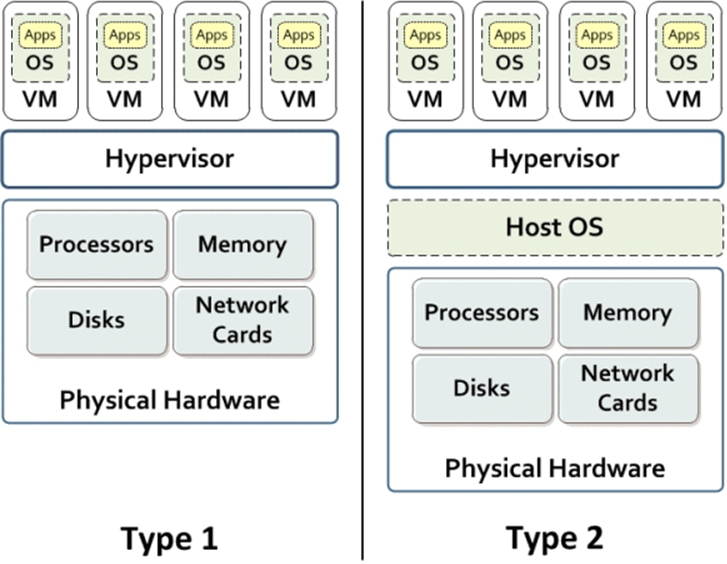
\includegraphics[scale=0.4]{afbeelding/hypervisors.png}}
\caption{Type 1 hypervisor in vergelijking met een type 2 hypervisor \citep{hypervisors}}
\label{fig:hypervisors}
\end{figure}

Met virtualisatie is het mogelijk om van één computer meerder computers te maken.
Dit kan bereikt worden door gebruik te maken van een speciaal programma (een hypervisor).
Volgens \citet{fenn2008evaluation} bestaan er twee types hypervisors (zie Figuur~\ref{fig:hypervisors}):
\begin{itemize}
\item \textbf{Type 1} hypervisors zorgen voor een directe interface naar de host hardware.
Er is typisch één virtuele machine met speciale privileges die de andere virtuele machines onderhoudt.
\item \textbf{Type 2} hypervisors draaien als een normaal programma in het host besturingssysteem.
Iedere virtuele machine draait dan als proces in het host besturingssysteem.
\end{itemize}

Een virtuele machine bevat een volledig besturingssysteem.
Een gevolg hiervan is dat het uitvoeren van handelingen (zoals opstarten, afsluiten, kopiëren, \ldots) lang duren.
Hiernaast moet tijdens het instellen van een virtuele machine een volledig besturingssysteem geïnstalleerd worden.
De tijd die nodig is om een VM in te stellen neemt hierdoor drastisch toe.
Aangezien een virtuele machine een volledig besturingssysteem omvat, heeft deze ook de resources nodig om correct te kunnen functioneren.
Om verschillende virtuele machines naast elkaar te kunnen laten draaien, moet de host voldoende RAM, CPU en harde schijf ruimte hebben.
Door gebruik te maken van een virtuele machine wordt een veilige omgeving gecreëerd maar dit neemt kostbare tijd en resources in beslag.

\begin{figure}[!ht]
\centering
\makebox[0pt]{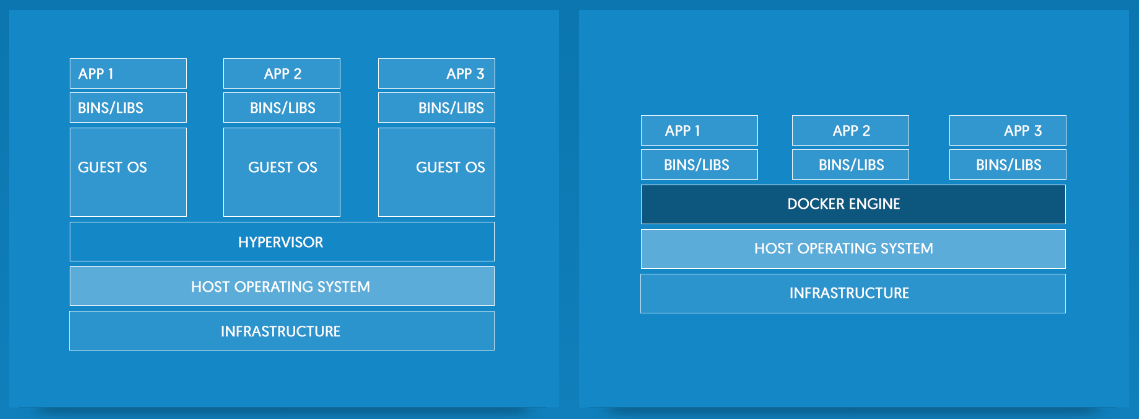
\includegraphics[scale=0.5]{afbeelding/dockerVsVM.png}}
\caption{Architectuur van Virtuele Machine ten opzichte van Docker \citep{dockerMain}}
\label{fig:VMvsDocker}
\end{figure}

\subsection{Docker}\label{sec:docker}
Virtualisatie is niet de enige techniek die gebruikt kan worden om rollbacks te vermijden.
Docker containers is een technologie waarmee een stuk software wordt ingepakt in een volledig filesysteem dat alle benodigdheden bevat om correct te functioneren.
Hierdoor zal de software overal op eenzelfde manier draaien, ongeacht de omgeving \citep{dockerMain}.
Docker containers zijn niet hetzelfde als virtuele machines.
In \citep{dockerEbook} worden virtuele machines voorgesteld als huizen terwijl Docker containers worden voorgesteld als appartementen.
De huizen staan volledig op zichzelf en bieden bescherming tegen ongewenste gasten.
Ze hebben een eigen infrastructuur met hun eigen water, verwarming, \ldots .
Hiernaast zal ieder huis op zijn minste een badkamer, living, slaapkamer en keuken hebben.
Het vinden van een klein huis is een ganse klus en vaak zal een huis meer bevatten dan nodig is want dat komt door de manier waarop huizen gebouwd worden.

Appartementen bieden ook bescherming tegen ongewenste gasten, maar zij zijn gebouwd rond een gemeenschappelijke infrastructuur.
Het appartementsgebouw biedt gemeenschappelijk water, verwarming, \ldots  aan, aan elk appartement.
Elk appartement kan van grootte verschillen.
Er bestaan kleine appartementen maar ook grote met meerder slaapkamers.
Men huurt enkel hetgeen nodig is.

In Figuur~\ref{fig:VMvsDocker} zijn de architecturen van virtuele machines en Docker terug te vinden.
Het verschil tussen beiden wordt al snel duidelijk.
Een virtuele machine zal typisch de applicatie, de nodige binaries en bibliotheken en een volledig besturingssysteem bevatten.
Een container bevat de applicatie en de verschillende dependencies maar de kernel wordt gedeeld met alle andere containers en gedragen zich als een geïsoleerd proces in de user space van het host besturingssysteem.

\citet{chamberlain2014using} bespreken kort hoe Docker werkt.
Docker is een platform dat gebruik maakt van de Linux Containers (LXC de user-space control package voor Linux Containers) om software te encapsuleren.
LXC is een virtualisatietechniek waarmee virtuele omgevingen in Linux opgebouwd kunnen worden.
De containers zullen processen van elkaar gescheiden houden zodat een proces een ander niet kan beïnvloeden \citep{merkel2014docker}.
Docker zal de LXC software uitbreiden waardoor deployment, distributie en versioning mogelijk wordt.
Naast LXC gebruikt Docker AuFS (Advanced Multi-Layered Unification Filesystem) als het filesysteem voor de containers.
Doordat het filesysteem gelaagd is, is het mogelijk om verschillende filesystemen over elkaar te leggen.

\citet{merkel2014docker} vergelijkt de twee virtualisatie technieken.
Bij virtuele machines moet voor iedere virtuele machine een besturingssysteem geïnstalleerd worden.
Al deze besturingssystemen verbruiken RAM, CPU en bandbreedte.
Containers zullen piggybacken op het bestaande host besturingssysteem.
Hierdoor zal het resource gebruik efficiënter zijn.
Een container is goedkoop waardoor het creëren en verwijderen van containers een snelle operatie.
Dit komt omdat er enkel een proces moet afgesloten worden in tegenstelling tot het afsluiten van een volledig besturingssysteem.
Een voordeel van de VMs ten opzichte van Docker is hun maturiteit.
VMs bestaan langer en hebben zichzelf kunnen bewijzen in verschillende situaties.

\section{Deployment strategieën}\label{sec:deployment}
%%% TODO herschrijven
Voordat software bij een gebruiker geïnstalleerd of geüpdatet kan worden, moet de software eerst bij de gebruiker geraken.
Er kan op twee manieren naar dit proces gekeken worden:
\begin{itemize}
\item Wat wordt er precies verzonden naar de gebruiker?
\item Wie krijgt de software als eerste?
\end{itemize}
In de volgende secties worden deze twee verschillende focussen verder besproken.

\subsection{Data focus}
\citet{deploymentMethods} haalt drie methodes aan om software te deployen:
\begin{itemize}
\item disk image-based deployment
\item behavior-based deployment
\item package-based deployment
\end{itemize}
Bij disk image-based deployment worden de software en het besturingssysteem op eenzelfde moment naar de target node verzonden.
Er zullen verschillende image-servers aanwezig zijn die elk een service aanbieden.
Zo zal de image-server van software A een andere image-server zijn dan de image-server die software B gebruikt.
Het voordeel van deze strategie is dat, zolang de hardware en software vereisten voldaan zijn, de deployment bestaat uit een simpele read-write operatie.
Maar, zoals \citet{deploymentMethods} al aangeeft, is deze methode niet flexibel.
Enkel software die op voorhand werd geconfigureerd op de image-server kan worden gedeployed.
Gebruikers met speciale noden kunnen moeilijk worden geholpen.
Voor Televic is flexibiliteit een hoofddoelstelling.
Iedere node bevat verschillende hardware en is verschillend geconfigureerd.
Een disk image-based deployment zal hierdoor niet gebruikt kunnen worden.
Het basisidee achter behavior-based deployment is het opnemen van de schijfoperaties tijdens het deployen.
Als geweten is welke bestanden aangepast, gecreëerd zijn, ... dan kan het proces nagebootst worden op andere nodes \citep{deploymentMethods}.
Zo een proces nabootsen is moeilijk.
Kerneloperaties moeten getraceerd worden.
Deze methode biedt een verhoogde flexibiliteit aan ten opzichte van de disk image-based deployment maar dit is nog niet voldoende om deployments uit te voeren die uniek zijn per node.
De laatste techniek die \citet{deploymentMethods} aan haalt is package-based deployment.
Met behulp van een batch file, waarin alle nodige commando's aanwezig zijn, kan een installatie pakket gedeployed worden naar een target node.
Door het gebruik van een batch file wordt de flexibiliteit van de deployment verhoogd.

\subsection{User focus}
De geproduceerde software moet bij verschillende gebruikers terecht komen.
Een eenvoudige oplossing zou zijn dat slechts één gebruiker per keer geholpen wordt en dat iedere gebruiker zijn beurt afwacht.
Zo'n oplossing is misschien doenbaar mochten slechts een handvol gebruikers de applicatie nodig hebben maar dit is vaak niet het geval.
\citet{patterson2008data} haalt verschillende argumenten aan voor het distribueren van deze service en haalt enkele punten aan (betrouwbaarheid, bandbreedte en lage wachttijden) waar rekening mee moet gehouden worden alvorens een ontwerpbeslissing genomen wordt.
Zoals \citet{patterson2008data} aanhaalt, is het belangrijk dat alle gebruikers ten alle tijden de service kunnen gebruiken.
Hiernaast moet er rekening gehouden worden met de deployment strategie.
\citet{munch2012software} spreken over verschillende strategieën om software uit te brengen:
\begin{itemize}
\item \emph{Big-bang}: iedere gebruiker van de applicatie zal op eenzelfde moment overschakelen van de oude naar de nieuwe software. 
Hierdoor wordt vermeden dat verschillende afdelingen met een andere versie van de software werken. 
Een nadeel is dat voldoende support aanwezig moet zijn om mogelijke problemen op te lossen.
\item \emph{Gefaseerd}: de nieuwe software zal bij een gefaseerde deployment enkel toegepast worden in specifiek geselecteerde projecten.
Als deze strategie voor een verlengde periode wordt toegepast, zullen verschillende versies van de software continu aanwezig zijn onder de gebruikers.
\end{itemize}
Aan beide strategieën zijn zowel voor- en nadelen gekoppeld.
Zo zal de big-bang strategie niet voordelig zijn om uit te voeren als de gebruikers verspreid zitten over de wereld.
Door het tijdsverschil zal de deployment bij sommige gebruikers plaatsvinden tijdens de werkuren en bij anderen midden in de nacht.
Het voordeel van de big-bang strategie is dat alle doelsystemen op een korte periode omgeschakeld worden naar de nieuwe versie van de applicatie. 
Het gebruik van de gefaseerde strategie kan het probleem met de tijdszones omzeilen maar deze strategie is ook niet ideaal aangezien het omschakelen van de software naar de nieuwe versie lang kan duren.
Een hybride oplossing is hier dus aangewezen.

\section{Architecturen}
Tot op heden werd vooral gekeken naar mogelijke technologieën en tools die gebruikt kunnen worden voor het verspreiden van software.
In de komende secties worden enkele architecturen aangehaald die ook een oplossing bieden voor het verspreiden van software.
Met een architectuur is het mogelijk om zelf verscheidene ontwerp- en implementatiebeslissingen te nemen.
Zo ligt de programmeertaal niet vast en kan een taal gekozen worden die besturingssysteem onafhankelijk is.
In de volgende secties wordt vooral gekeken welke architecturen een schaalbare oplossing bieden voor het deploymentproces.

\subsection{Client-server architectuur}
\citet{encyclo} beschrijft de client-server architectuur als een architectuur van een computernetwerk waarin verscheidene clients services van een gecentraliseerde server opvragen en ontvangen.
De client computers dienen als interface voor de gebruikers om services op te vragen en het resultaat van de server weer te geven.
De architectuur bevordert het ontwerpen van systemen die modulair, flexibel en uitbreidbaar zijn door eventuele data, resources of computeroperaties te integreren, te organiseren en aan te bieden als een service \citep{adler1995distributed}. 
Figuur~\ref{fig:clientServer} geeft de client-server architectuur weer.

\begin{figure}[!ht]
\centering
\makebox[0pt]{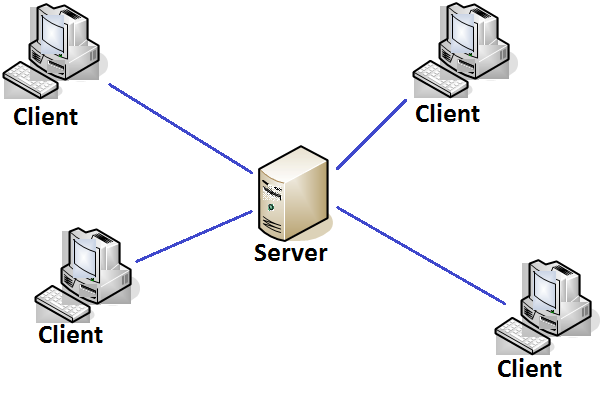
\includegraphics[scale=0.7]{afbeelding/clientServerSimple.png}}
\caption{Client-server architectuur}
\label{fig:clientServer}
\end{figure}

Een voordeel van de client-server architectuur is dat clients zich niet moeten bezig houden met het verwerken van data.
Clients kunnen zich focussen op het opvragen van informatie van de computergebruikers en de server en clients kunnen zich focussen op het weergeven van deze data \citep{oracleClientServer}.
Doordat de architectuur bestaat uit een server die verscheidene requests van clients afhandelt, is deze server ook de zwakke schakel in de architectuur.
Bij het uitvallen van de server, is het niet mogelijk om het netwerk in stand te houden.
Een netwerk waar slechts één server in aanwezig is, bevordert dan ook niet de schaalbaarheid.
Hiernaast wordt de communicatie tussen de client en de server geïnitieerd door de client die een service van de server wilt gebruiken.
Aangezien het doel het verspreiden van software vanuit de server is, moet het mogelijk zijn om vanuit de server updates te verspreiden.
\citet{mesbah2008component} leggen uit dat het client-geïnitieerde afhaalmodel inefficiënt is voor real-time event notificaties.
Dit is een groot nadeel aan deze architectuur aangezien het mogelijk moet zijn om vanuit een softwareproducent de verscheidene clients op de hoogte te brengen van bijvoorbeeld nieuwe software die beschikbaar is.
Een oplossing voor dit probleem is het hanteren van een push-gebaseerd model waarbij de server aanpassingen uitzendt naar alle clients.

%Volgens \citet{micro} is het mogelijk om een applicatie in te delen in drie logische groepen of ook wel lagen.
%Het gebruik van een laag stelt de ontwerper in staat om verscheidene taken van elkaar te onderscheiden waardoor het eenvoudiger is om een laag te ontwerpen die herbruikbaar is.
%Figuur~\vref{fig:threeLayer} toont welke drie basis lagen gebruikt worden om de architectuur op te bouwen.
%Hierbij wordt de presentatie laag gebruikt om alle functionaliteiten die instaan voor het onderhouden van de gebruikersinteracties met het systeem te groeperen.
%De bussiness laag encapsuleert alle relevante bussiness logica die de kern van het systeem bevat.
%De laatste laag, de data laag, voorziet toegang tot verschillende databronnen binnen in het netwerk maar ook daarbuiten.
% 
%\begin{figure}[!ht]
%\centering
%\makebox[0pt]{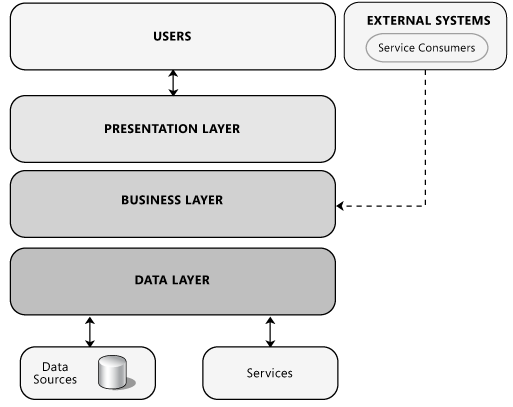
\includegraphics[scale=0.7]{afbeelding/threeLayer.png}}
%\caption{Drie lagen architectuur \citep{micro}}
%\label{fig:threeLayer}
%\end{figure}
%
%Het gebruik van deze architectuur gaat gepaard met enkele voordelen.
%Zo zorgt het gebruik van lagen ervoor dat het aanpassen van één laag amper of geen invloed heeft op de andere lagen.
%Verder zorgt het opdelen van de applicatie en database functionaliteiten ervoor dat beter load balancing kan worden toegepast.
%In de verschillende lagen is het mogelijk om voldoende veiligheidsmaatregelen toe te passen zonder de gebruikers te hinderen.
%Figuur~\ref{fig:threeLayerExample} geeft weer op welke wijze de architectuur gebruikt kan worden om een applicatie hosten.
%
%\begin{figure}[!ht]
%\centering
%\makebox[0pt]{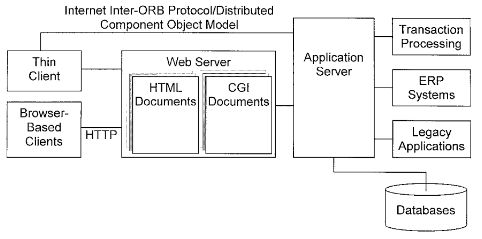
\includegraphics[scale=1]{afbeelding/threeLayerExample.png}}
%\caption{Voorbeeld van een drie lagen architectuur \citep{hanson2000client}}
%\label{fig:threeLayerExample}
%\end{figure}
%
%Het verspreiden van software kan met deze architectuur op een eenvoudige manier gerealiseerd worden.
%Clients kunnen verbinding maken met een web server.
%Vanuit een browser is het vervolgens mogelijk om verschillende softwarecomponenten te combineren tot één geheel die naar de gebruiker verscheept wordt voor installatie.
%De web server zorgt voor de nodige flexibiliteit waarbij het voor een gebruiker mogelijk is om vanuit een browser de te installeren software zelf te selecteren.
%De software kan bij de gebruiker geraken maar de architectuur biedt geen mogelijkheden aan die toestaan om de software te installeren.
%Hiervoor is echter ondersteuning nodig die niet is opgenomen in de architectuur.
%Hiernaast laat de architectuur ook een groeiend aantal gebruikers toe.
%Iedere laag kan redundant gemaakt worden waarbij meerdere server van eenzelfde laag parallel naast elkaar kunnen draaien.
%De drie lagen architectuur voorziet voldoende flexibiliteit en schaalbaarheid maar logica voor het opvangen van fouten tijdens het installatieproces en updateproces is niet aanwezig.

\subsection{Software dock architectuur}\label{sec:softwareDock}
\citet{hall1999cooperative} bespreken een interessante architectuur die gebruikt kan worden voor het verspreiden van software.
Het Software Dock research project creëerde een raamwerk om de samenwerking tussen software producenten en gebruikers te verbeteren.
In Figuur~\ref{fig:softwareDock} wordt de ontworpen architectuur voorgesteld.
Er worden twee verschillende componenten gedefinieerd waarmee de producenten en gebruikers voorgesteld worden.
In de architectuur worden de verschillende producenten voorgesteld aan de hand van een release dock en worden de gebruikers voorgesteld als een field dock.
Aan deze docks worden verschillende agenten gekoppeld.
Elke agent hoort typisch bij één stap uit de software levenscyclus die besproken werd in Sectie~\ref{sec:softwareLevenscyclus}.
Naast de verschillende docks wordt ook een wide-area eventsysteem gedefinieerd.
Met dit systeem wordt de communicatie tussen de docks geregeld.
\citet{hall1997architecture} bespreken in detail hoe de Software Dock architectuur gebruikt kan worden voor het verspreiden van software.

\begin{figure}[!ht]
\centering
\makebox[0pt]{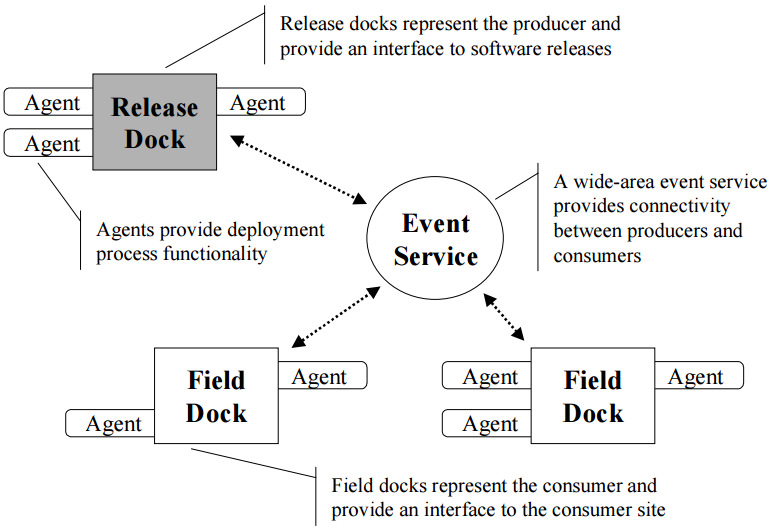
\includegraphics[scale=0.5]{afbeelding/softwareDockArchitectuur.png}}
\caption{Software Dock Architectuur \citep{hall1999cooperative}}
\label{fig:softwareDock}
\end{figure}

De release dock is een softwarecomponent die zich bevindt bij de softwareproducent.
De release dock biedt een release-repository aan waaruit de gebruikers de applicaties selecteren voor deployment.
In de release dock wordt ieder release semantisch beschreven aan de hand van een Deployable Software Description file.
Dit bestand bevat onder andere:
\begin{itemize}
\item \textbf{Assertion}: deze worden gebruikt om beperkingen die aan de gebruikerskant waar moeten te beschrijven.
Als niet aan deze beperkingen voldaan wordt, zal het deploymentproces falen.
\item \textbf{Afhankelijkheden}: deze worden gebruikt om beperkingen van de release te beschrijven.
Als deze niet voldaan zijn aan de gebruikerskant dan kunnen nog oplossingen gevonden worden.
Bijvoorbeeld door additionele software te installeren kan aan de beperking voldaan worden.
\item \textbf{Configuratie}: deze zorgt voor een beschrijving van de software die wordt uitgegeven.
Hierbij horen bijvoorbeeld varianten en aangepaste versies.
\end{itemize}
Elke release wordt vergezeld door enkele agents die de semantische betekenis lezen en zo de deployment kunnen uitvoeren.
Aan de hand van interfaces kunnen de agents aan de services en inhoud van de release dock.
Bij het wijzigen van een software release zal de release dock verschillende events afvuren.
Agenten kunnen zich inschrijven voor deze events en weten zo wanneer bepaalde handelingen uitgevoerd moeten worden \citep{hall1999cooperative}.

De field dock dient als een interface naar de gebruikerskant toe.
Deze interface biedt informatie over de resources en configuratie van het gebruikerssysteem.
Op basis van deze informatie wordt een context opgebouwd waarin de releases van de resource dock worden gedeployed.
De agenten die horen bij een release, docken zichzelf in de field dock en kunnen aan de hand van deze interface het gebruikerssysteem ondervragen.
Aangezien kritische client-side informatie op een gestandaardiseerde wijze aangeboden wordt, met behulp van een geneste collectie van pair-values die een hiërarchie vormen, kan de installatie van de software gepersonaliseerd worden \citep{hall1999cooperative}.

\subsubsection{Communicatie}\label{sec:event}
%%% TODO
Een belangrijk onderdeel van de software dock architectuur is de event service.
Deze handelt de communicatie af tussen de verschillende docks en is een spilfiguur in de architectuur.
Aan de hand van \citet{pietzuch2002hermes} en \citet{carzaniga2001design} is het mogelijk om een bespreking te geven over hoe de event service geïmplementeerd kan worden.

De meeste middleware systemen zijn invocation-based systemen waarbij het request/response paradigma gebruikt wordt om de communicatie tussen client en server te onderhouden.
Een client verzoekt een service van de server, waar de server vervolgens op antwoordt.
Het toepassen van deze strategie is doenbaar in een omgeving met een beperkt aantal clients en servers.
Om een grootschalig netwerk op te bouwen en om te kunnen gaan met een dynamische omgeving moet een andere manier van communiceren gebruikt worden.
Publish/subscribe systemen bieden een oplossing voor deze problemen.
Clients, event subscribers, tonen hun interesse voor een bepaald onderwerp en servers, event publishers, produceren een event die naar alle geïnteresseerden wordt doorgestuurd.
Een algemeen voorbeeld is terug te vinden in Figuur~\ref{fig:pubsubArchi}.
Door deze manier van communiceren te hanteren, ontstaat een natuurlijke ondersteuning voor many-to-many relaties tussen de clients en servers.
De twee worden ook van elkaar ontkoppeld.
Voor de client maakt het niet uit welke publisher de producent is van een event.
Hiernaast moet de server niet weten wie allemaal de events ontvangt die hij produceert \citep{pietzuch2002hermes}.

\begin{figure}[!ht]
\centering
\makebox[0pt]{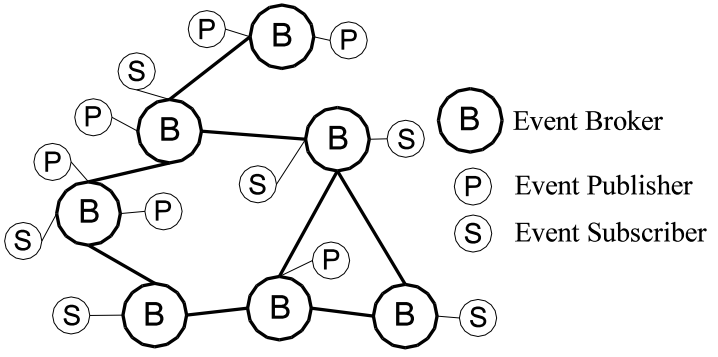
\includegraphics[scale=0.5]{afbeelding/pubsubArchi.png}}
\caption{Broker netwerk \citep{pietzuch2002hermes}}
\label{fig:pubsubArchi}
\end{figure}

Een naïeve aanpak, volgens \citet{carzaniga2001design}, is het gebruiken van één centrale server waar alle subscripties worden bijgehouden, waar alle events toekomen, waar de bestemming van het event beslist wordt en waar het event wordt doorgestuurd naar de gepaste subscribers.
Deze strategie is eenvoudig te implementeren maar deze werkt de schaalbaarheid tegen.
Dit was ook al duidelijk in Figuur~\ref{fig:pubsubArchi} waar verschillende ``Brokers'' aanwezig zijn.
Het is belangrijk om stil te staan bij enkele ontwerp beslissingen zodanig dat de service die in Figuur~\ref{fig:pubsubService} zichtbaar is, implementeerbaar is.

\begin{figure}[!ht]
\centering
\makebox[0pt]{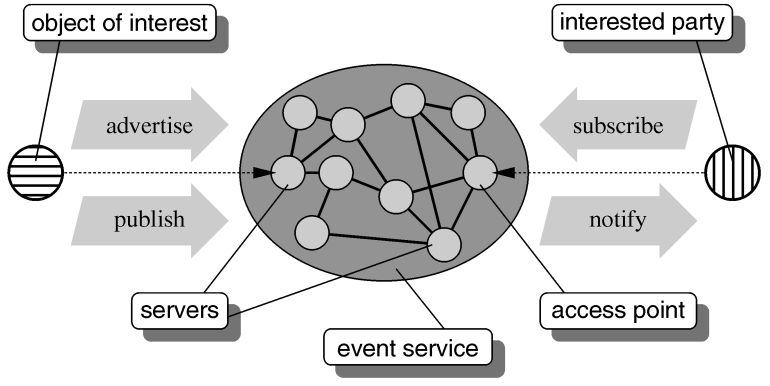
\includegraphics[scale=0.5]{afbeelding/pubsub.png}}
\caption{Publish/Subscribe service \citep{carzaniga2001design}}
\label{fig:pubsubService}
\end{figure}

Naast de architectuur is het belangrijk om te weten wat wordt verzonden en op welke manier.
\citet{carzaniga2001design} halen een structuur aan waarin een event beschreven wordt als een set van attributen.
Ieder attribuut bestaat uit een type, naam en waarde.
De naam van een attribuut is een string en het type komt uit een set van primitieven die terug gevonden worden bij de meeste hedendaagse programmeertalen.
Een voorbeeld van zo'n event is terug te vinden in Figuur~\ref{fig:pubsubNot}

\begin{figure}[!ht]
\centering
\makebox[0pt]{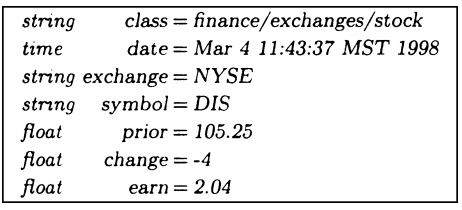
\includegraphics[scale=0.5]{afbeelding/pubsubNot.png}}
\caption{Publish/Subscribe Event \citep{carzaniga2001design}}
\label{fig:pubsubNot}
\end{figure}

\section{Technologieën voor software packaging}\label{sec:technologieen}
In de vorige secties werden oplossingen gezocht voor het verspreiden van software naar verschillende gebruikers.
Hierbij werd vooral rekening gehouden met de wijze waarop de software verzonden wordt.
Er werd nagegaan of een oplossing zorgde voor een schaalbare architectuur die mogelijkheden biedt naar de toekomst toe.
In wat volgt wordt niet meer gekeken naar hoe de software bij de gebruiker raakt maar wat er bij de gebruiker raakt.

Implementaties in verschillende programmeertalen, verschillende datarepresentatieformaten of incompatibele runtime-environments kunnen aan de basis liggen van een lastige integratie van computerprogramma's.
Door gebruik te maken van additionele software, wordt het mogelijk om het gat tussen de verschillen te overbruggen  \citep{callahan1998software}.
Het Python testraamwerk is een verzameling van verschillende drivers en bibliotheken elk met een eigen implementatie.
Door additionele software toe te voegen is het mogelijk dat verschillende software ``pakketten'' op een gelijkaardige manier behandeld worden.
In wat volgt zullen verschillende technologieën en tools besproken worden die ervoor zorgen dat verschillende software ``pakketten'' een geheel vormen.
Dit geheel kan vervolgens verzonden worden naar de gebruikers waar de software geïnstalleerd moet worden.

Om de verschillende technologieën te vergelijken werd een algemeen testscenario uitgedacht.
Er moet een geheel gemaakt worden waarmee twee verschillende pakketten (die drivers en bibliotheken moeten voorstellen) geïnstalleerd moeten worden.
Hierna werd er onderzocht hoe één van de twee pakketten geüpdatet kon worden.
Door de technologieën te onderwerpen aan een test, wordt het mogelijk om de voor- en nadelen van iedere technologie te achterhalen.
Hiernaast wordt het ook mogelijk om de technologieën te vergelijken aangezien zij eenzelfde functionaliteit moeten voorzien.

%\begin{table}[]
%\centering
%\begin{tabular*}{\linewidth}{clll}
%\hline
%\multicolumn{4}{p{\linewidth}}{\centering \textbf{WiX Toolset}}                    \\ 
%\multicolumn{2}{p{0.5\linewidth}}{\centering Pro} & \multicolumn{2}{p{0.5\linewidth}}{\centering Cons} \\ \hline
%\multicolumn{2}{p{0.5\linewidth}}{Diepe integratie met Windows \par Mogelijkheid om externe executables te includeren}   & \multicolumn{2}{p{0.5\linewidth}}{XML structuren zorgt voor veel overhead \par Niet cross-platform}    \\ \hline
%\multicolumn{4}{p{\linewidth}}{\centering \textbf{NSIS}}                           \\ 
%\multicolumn{2}{p{0.5\linewidth}}{\centering Pro} & \multicolumn{2}{p{0.5\linewidth}}{\centering Cons} \\ \hline
%\multicolumn{2}{p{0.5\linewidth}}{Scripting taal \par Verschillende plug-ins beschikbaar}   & \multicolumn{2}{p{0.5\linewidth}}{ Niet cross-platform \par Geen structuur voor packages}    \\ \hline
%\multicolumn{4}{p{\linewidth}}{\centering \textbf{Chocolatey}}                     \\ 
%\multicolumn{2}{p{0.5\linewidth}}{\centering Pro} & \multicolumn{2}{p{0.5\linewidth}}{\centering Cons} \\ \hline
%\multicolumn{2}{p{0.5\linewidth}}{Volledige deployment infrastructuur al aanwezig}   & \multicolumn{2}{p{0.5\linewidth}}{Niet cross-platform \par Command-line tool}    \\ \hline
%\multicolumn{4}{p{\linewidth}}{\centering \textbf{Qt Installer Framework}}         \\ 
%\multicolumn{2}{p{0.5\linewidth}}{\centering Pro} & \multicolumn{2}{p{0.5\linewidth}}{\centering Cons} \\ \hline
%\multicolumn{2}{p{0.5\linewidth}}{Cross-platform \par Mogelijkheid om externe executables te includeren}   & \multicolumn{2}{p{0.5\linewidth}}{XML structuren zorgt voor veel schrijfwerk \par Enkel Linux installer maken in Linux} \\ \hline
%\end{tabular*}
%\caption{Voor- en nadelen van de verschillende technologieën}
%\label{tab:voorNadelen}
%\end{table}

\subsubsection{WiX Toolset}
Windows installer XML Toolset is een set van build tools waarmee Windows Installer packages gemaakt worden met behulp van XML broncode.
De toolset is geschreven in C\# en heeft het .Net framework nodig om te kunnen functioneren.
Broncode wordt gecompileerd en vervolgens gelinkt om een executable te maken.
Met de toolset kunnen .msi installatie pakketten, .msm merge modules en .msp patches gecombineerd worden tot een Windows executabel \citep{wixToolset}.

Aan deze technologie zijn verschillende voor- en nadelen verbonden.
De WiX toolset is diep geïntegreerd met Windows waardoor er tijdens de installatie van software gebruik gemaakt kan worden van verscheidene functionaliteiten die bij Windows horen.
De WiX toolset maakt installers die uitsluitend bedoeld zijn voor de Windows installation engine.
Hierdoor worden verscheidene functionaliteiten eenvoudig te gebruiken, zoals het maken van uitzonderingen in de Windows Firewall.
Hiernaast kan tijdens het installatieproces rekening gehouden worden met externe installers.
Op deze manier is het mogelijk om verscheidene software pakketten te combineren tot één geheel.
Een fragment van de WiX toolset code is terug te vinden in Listing~\ref{list:wix}.
Door gebruik te maken van de Windows installation engine is het niet mogelijk om de executable te gebruiken in Linux omgevingen. 
Dit kan eventueel omzeild worden door het gebruik te maken van software zoals Wine \citep{amstadt1994wine}.
Als geen alternatieven aanwezig zijn, dan is deze strategie eventueel het overwegen waard.
WiX maakt gebruik van XML broncode om verschillende elementen te definiëren.
\citet{xmill} geeft al aan dat XML niet een van de meest efficiënte dataformaten is, maar het verhoogt de flexibiliteit wel.
Het creëren van een XML bestand met de hand is een langdradig en moeilijk werk.

\subsubsection{NSIS}
Nullsoft Scriptable Install System is een open source systeem waarmee Windows installers gemaakt kunnen worden.
Zoals de naam aangeeft, is NSIS script-based.
Hierdoor bevatten installers het nodige om verschillende installatietaken uit te voeren.
Door de grote gebruikersbasis is een grote hoeveelheid plug-ins en scripts beschikbaar.
Alle plug-ins en scripts kunnen op een eenvoudige manier aan een installer toegevoegd worden voor een verhoogde functionaliteit \citep{nsisMain}.

Met de scripting taal van NSIS is het mogelijk om eenvoudige installer te definiëren (een voorbeeld hiervan is terug te vinden in Listing~\ref{list:nsis}).
De scripting taal is intuïtiever te gebruiken in vergelijking met de XML bestanden van Wix Toolset en is dan ook een voordeel bij deze technologie.
Dankzij de grote hoeveelheid aan plug-ins die aanwezig zijn, is het eenvoudig om een installer te creëren met verschillende functionaliteiten.
De gecreëerde installer is een Windows executable en de opmerking gegeven bij de WiX Toolset is hier ook van toepassing en is dan ook een nadeel van deze technologie.
Het feit dat NSIS bedoeld is om eenvoudige installers te maken zorgt ervoor dat het niet mogelijk is om aparte pakketten te definiëren.
Ieder pakket kan wel een eigen configuratie hebben maar dit wordt allemaal toegevoegd aan één script.
Een grote hoeveelheid aan pakketten leidt tot wanorde.
NSIS biedt ook geen mogelijkheden aan om geïnstalleerde software up te daten.
Om die eigenschappen toe te voegen moet er beroep gedaan worden op andere software.

\subsubsection{Chocolatey \& apt-get}
Volgens \citep{chocoAbout} is Chocolatey een package mangager voor Windows net zoals apt-get voor Linux is.
Het is ontworpen als een gedecentraliseerd framework met als doel het snel installeren van applicaties en tools.
Chocolatey werd gebouwd boven op de NuGet infrastructuur gecombineerd voor het verspreiden van de packages en gebruikt PowerShell voor een gepersonaliseerde installatie.

Het grootste voordeel dat bekomen wordt bij het gebruiken van een package manager is het al bestaan van een deployment infrastructuur. 
Na het installeren van Chocolatey op de client kunnen alle nodige packages voor het framework geïnstalleerd worden.
Hiernaast kunnen scripts gekoppeld worden aan iedere package zodanig dat een aangepaste installatie mogelijk is.
Net zoals apt-get voor Linux, is Chocolatey te gebruiken in de command-line.
Dit is vooral een nadeel naar gebruiksvriendelijkheid toe aangezien er vanuit wordt gegaan dat de gebruikers amper tot geen ervaring hebben met de command-line in Windows/Linux.
Dit is echter eenvoudig op te lossen door het toevoegen van een grafische user interface.
Het grootste nadeel aan deze technologie is, net zoals de vorige opties, het niet cross-platform zijn.

\subsubsection{Qt Installer Framework}
Het Qt Installer Framework biedt een set van tools aan voor het creëren van installers op verschillende platformen.
Aan de hand van een set van pagina's wordt de gebruiker door het installatie-, update- en verwijderproces geleid.
Hierbij kunnen scripts gebruikt worden om het proces te vereenvoudigen \citep{qtDoc}.
Door een folder structuur op te bouwen zoals Figuur~\ref{fig:folder} kan het Qt installer framework een installer creëren die vervolgens op het doelsysteem uitgevoerd kan worden.

\begin{figure}[!ht]
\centering
\makebox[0pt]{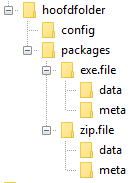
\includegraphics[scale=0.9]{afbeelding/folder.png}}
\caption{Folder structuur voor installer}
\label{fig:folder}
\end{figure}

De datafolder van een pakket bevat alle nodige databestanden die moeten uitgevoerd worden (zoals een executable of een zip archief).
De metafolder bevat een beschrijving van het pakket (zie voorbeeld in Listing~\ref{list:qtpakket}).
Hiernaast is ook een installatiescript aanwezig dat uitgevoerd wordt tijdens de installatie van het pakket zelf (zie Listing~\ref{list:qtscript}).
Met de installer informatie uit de config folder (zie Listing~\ref{list:qtinstaller}) weet het Qt installer framework voldoende om een executable te produceren die alle pakketten installeert aan de hand van de opgegeven installatiescripts.
Op deze wijze is het mogelijk om verschillende pakketten te combineren tot één geheel en ondertussen toch ieder pakket apart te behandelen.

Aan deze technologie zijn verschillende plus- en minpunten verbonden.
Het grootste voordeel van het Qt Installer framework is het cross-platform zijn.
Hierdoor is het mogelijk om installers te maken voor zowel Windows als Linux.
Een nadeel dat hieraan verbonden is, is dat een Linux installer enkel kan gemaakt worden in een Linux omgeving.
Het is niet mogelijk om een Linux installer te maken op een Windows systeem.
Hiernaast is het wel mogelijk om voor ieder pakket een aparte installatieprocedure te implementeren.

\subsection{Conclusie}
Tabel~\ref{tab:voorNadelen} geeft een overzicht van de besproken technologieën en de voor- en nadelen die aan iedere technologie gekoppeld zijn.
Hieruit wordt snel duidelijk dat geen enkele technologie enkele pluspunten bevat.
Naar het ontwerp van de applicatie toe, moet er rekening gehouden worden met alle voor- en nadelen die aan de technologieën gekoppeld zijn.
De beste technologie wordt gekozen of er wordt zelf software voor het combineren van pakketten ontworpen die gebaseerd is op deze technologieën.

\begin{table}[]
\centering
\resizebox{\textwidth}{!}{%
\begin{tabular}{|c|l|l|}
\hline
\multicolumn{1}{|l|}{}                                                                  & \multicolumn{1}{c|}{Voordeel}                                            & \multicolumn{1}{c|}{Nadeel}                                       \\ \hline
\rowcolor[HTML]{C0C0C0} 
\cellcolor[HTML]{C0C0C0}                                                                & Diepe integratie met Windows                                             & XML structuren zorgt voor veel overhead                           \\
\rowcolor[HTML]{C0C0C0} 
\multirow{-2}{*}{\cellcolor[HTML]{C0C0C0}WiX Toolset}                                   & Mogelijkheid om externe executables te includeren                        & Niet cross-platform                                               \\ \hline
\rowcolor[HTML]{FFFFFF} 
\cellcolor[HTML]{FFFFFF}                                                                & Scripting taal                                                           & Geen structuur voor packages                                      \\
\rowcolor[HTML]{FFFFFF} 
\multirow{-2}{*}{\cellcolor[HTML]{FFFFFF}NSIS}                                          & Verschillende plug-ins beschikbaar                                       & Niet cross-platform                                               \\ \hline
\rowcolor[HTML]{C0C0C0} 
\cellcolor[HTML]{C0C0C0}                                                                & Volledige deployment infrastructuur al aanwezig                          & Command-line tool                                                 \\
\rowcolor[HTML]{C0C0C0} 
\multirow{-2}{*}{\cellcolor[HTML]{C0C0C0}Chocolatey}                                    &                                                                          & Niet cross-platform                                               \\ \hline
\rowcolor[HTML]{FFFFFF} 
\cellcolor[HTML]{FFFFFF}{\color[HTML]{000000} }                                         & {\color[HTML]{000000} Cross-platform}                                    & {\color[HTML]{000000} XML structuren zorgt voor veel schrijfwerk} \\
\rowcolor[HTML]{FFFFFF} 
\multirow{-2}{*}{\cellcolor[HTML]{FFFFFF}{\color[HTML]{000000} Qt Installer Framework}} & {\color[HTML]{000000} Mogelijkheid om externe executables te includeren} & {\color[HTML]{000000} Enkel Linux installer maken in Linux}       \\ \hline
\end{tabular}%
}
\caption{Voor- en nadelen van de verschillende technologieën}
\label{tab:voorNadelen}
\end{table}

%%% TODO Schrijven over het gebruiken van Windows .exe in Linux? Bijvoorbeeld hoe Wine misschien een oplossing is?

%%% TODO Schrijven over de test setup voor de verschillende technologieën die gebruikt is tijdens de stage?
